\section{Conclusion and Future Developments}
\label{sec:model_development}
% copio il blocco delle conclusione e sviluppi futuri, togliendo rd, rl
% etc. se è troppo lungo il tutto dovremo togliere qualcosa qua e là.

We developed an anatomical morphometric model of the newborn
lung. Using a CT scan of a newborn infant, we extracted the centreline
and the lobe surfaces (see \cref{fig:major_airways_xz}).

%% ex Figure 7
\begin{figure}[]\centering
  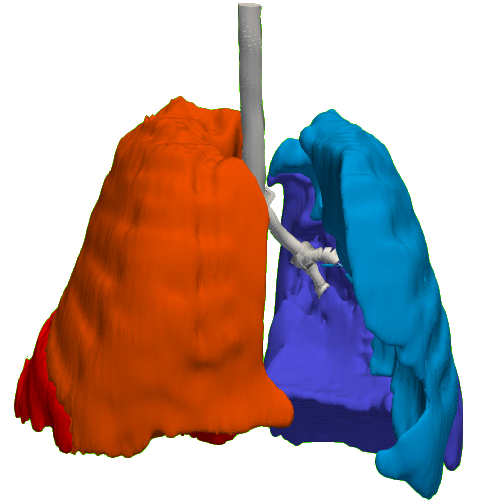
\includegraphics[width=.45\textwidth]{major_airways_xz.png}
  \caption{Major Airways and Lobes segmentations.  Cyan: Upper Left
    Lung; Blue: Lower Left Lung; Orange: Upper Right Lung; Red: Lower
    Right Lung.}
  \label{fig:major_airways_xz}
\end{figure}

We then reconstructed the anatomy of the missing airways using a
statistical algorithm originally proposed for adult lungs, which we
adapted for the newborn lung. This algorithm assigned airway diameters
based on proportions measured in the newborn lung (see
\cref{fig:complete_airways_xz}).

%% ex Figure 7a
\begin{figure}[]\centering
  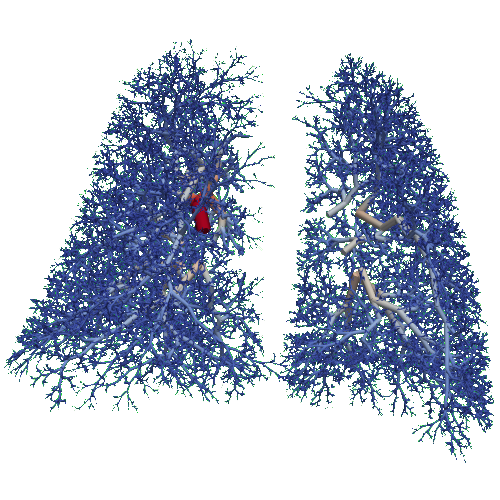
\includegraphics[width=.45\textwidth]{complete_airways_xz.png}
  \caption{Complete Airways generated by Chaste User Project (major
    airways are here excluded).  They are color-coded by their radii.}
  \label{fig:complete_airways_xz}
\end{figure}

We implemented a mechanical analog of the airway and acini in
Julia. This model accounts for changes related to aeration at birth,
allowing the simulation of the flow of fetal fluid toward the
periphery as air enters the airways.  The model incorporates changes
in resistance (R) and compliance (I), as well as capillary pressure
developed in the airways at the fluid-air interface. Testing on a
subset of the anatomical tree yielded consistent results (see
\cref{fig:mechanical_results_10,fig:mechanical_results_8}),
demonstrating the model's ability to simulate the phenomena involved
in lung aeration. Future developments will include simulating the
entire airway tree and analyzing the time required for full network
simulation.

%% ex Figure 8
\begin{figure}[]\centering
  \subfloat[][Airways voltages]{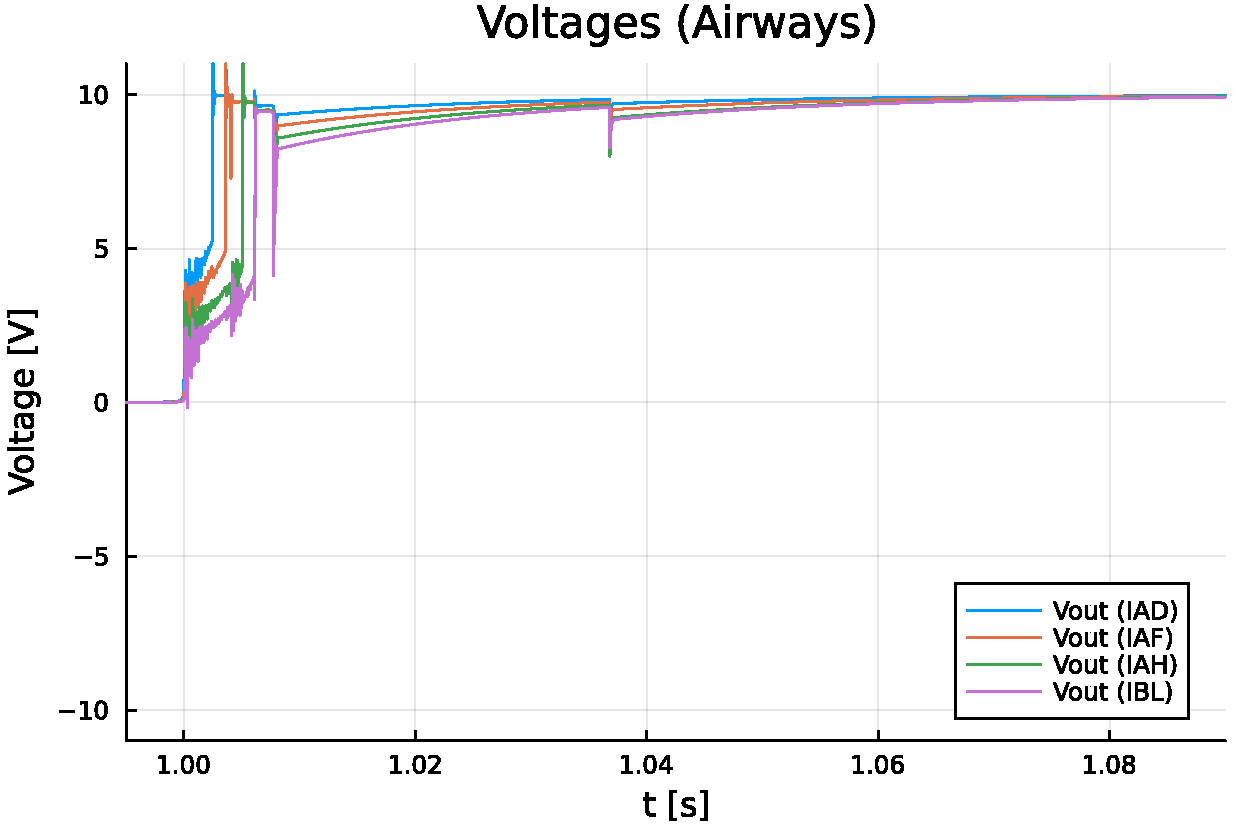
\includegraphics[width=.45\textwidth]{airways_voltages_10.pdf}}\\
  \subfloat[][Acini voltages]{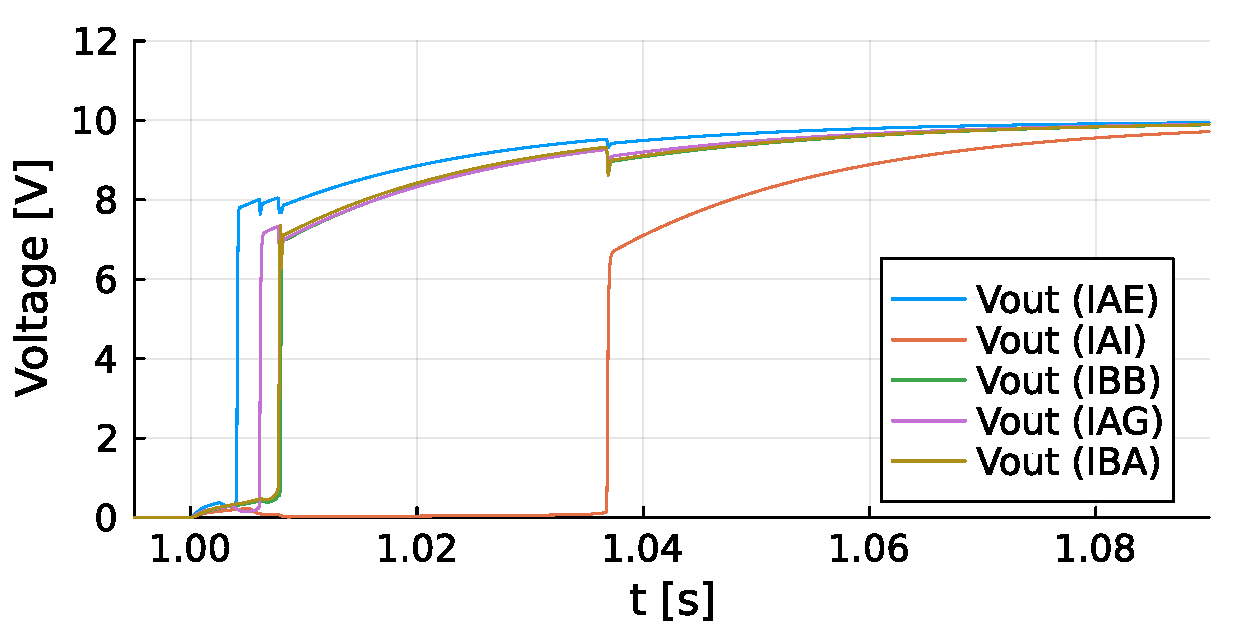
\includegraphics[width=.45\textwidth]{acini_voltages_10.pdf}}
  \caption{(Electrically equivalent) mechanical simulation for acini
    and airways.  The step amplitude is 10V.}
  \label{fig:mechanical_results_10}
\end{figure}

%% ex Figure 9
\begin{figure}[]\centering
  \subfloat[][Airways voltages]{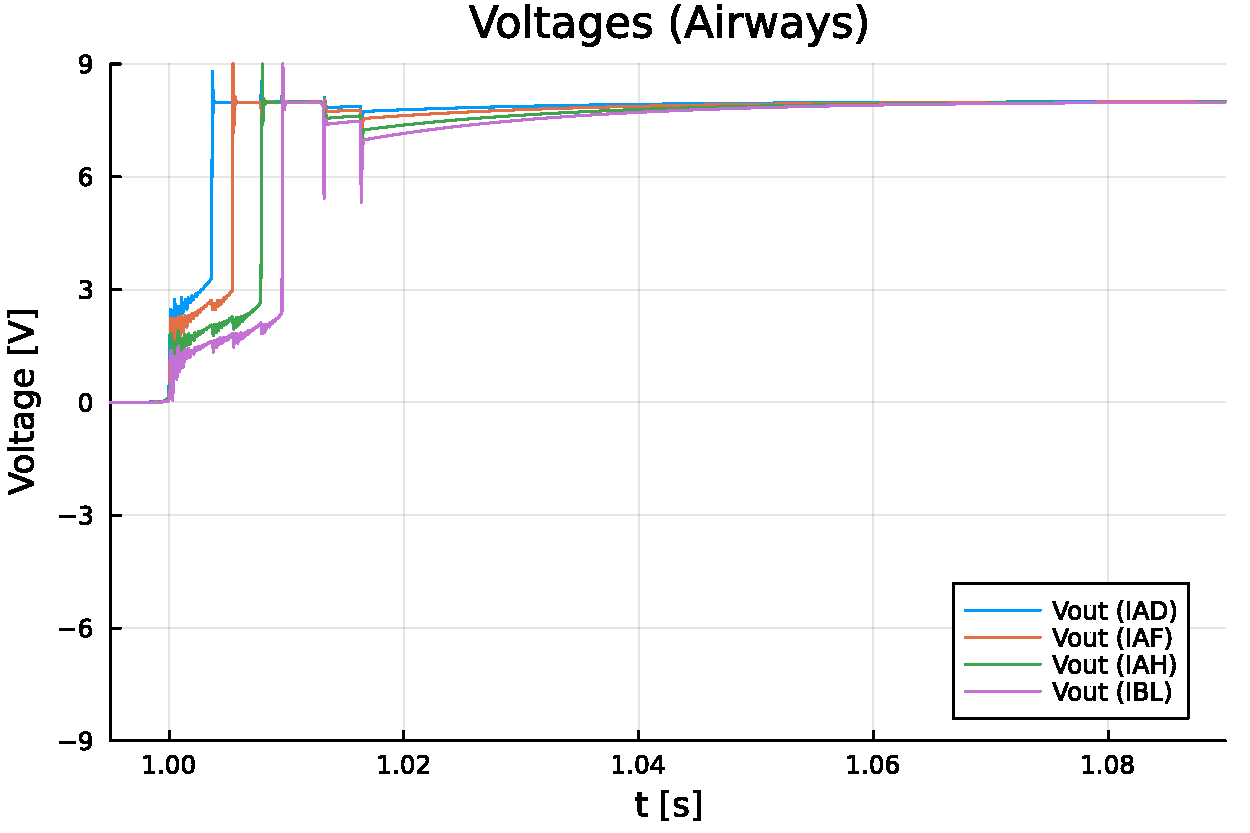
\includegraphics[width=.45\textwidth]{airways_voltages_8.pdf}}\\
  \subfloat[][Acini voltages]{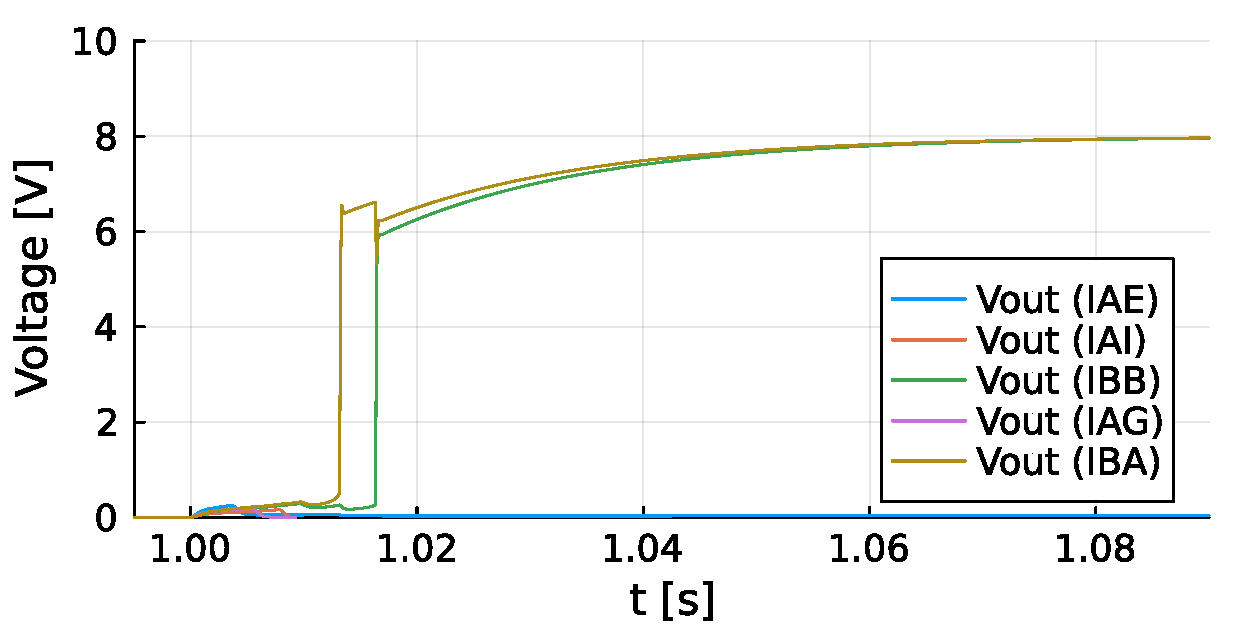
\includegraphics[width=.45\textwidth]{acini_voltages_8.pdf}}
  \caption{(Electrically equivalent) mechanical simulation for acini
    and airways.  The step amplitude is 8V.}
  \label{fig:mechanical_results_8}
\end{figure}

%%% Local Variables:
%%% mode: LaTeX
%%% TeX-master: "../Executive"
%%% End:
